\documentclass{beamer}
\usepackage{umnslides}
\usepackage{bibentry}
\usepackage[backend=biber,style=ieee, citestyle=authoryear]{biblatex}
\bibliography{bibfile.bib}

\title{Short-Baseline Neutrino Program}
\date{December 2023}
\author{Shardul Rao}
% \logo{
\includegraphics[height=1cm]{umn-logo.png}}

\AtBeginSection[]
{
  \begin{frame}
    \frametitle{Outline}
    \tableofcontents[currentsection]
  \end{frame}
}

\begin{document}

\frame{\titlepage}
\normalsize

\section{Introduction to SBN}
\begin{frame}{Overview of SBN}
\begin{itemize}
    \item Three neutrino detectors at Fermilab \footnotesize[\cite{SBN-Paper}]\normalsize
    \vspace{0.5cm}
    \item Short-baseline
    \vspace{0.5cm}
    \item Currently ongoing
    \vspace{0.5cm}
    \item Motivated by LSND and MiniBooNE results
    \vspace{0.5cm}
    \item Precursor to DUNE
\end{itemize}

\begin{figure}
    
\includegraphics[width = 0.25\linewidth]{umn/sbn-logo.jpg}
    \label{fig:sbn-logo}
\end{figure}
\end{frame}

\section{Physics of SBN}
\begin{frame}{Neutrino Oscillations}
    \begin{itemize}
        \item Freely-travelling neutrinos can oscillate in flavor \footnotesize[\cite{neutrino-oscillations}]\normalsize
        \vspace{0.5cm}
        \item Oscillation is characterized by the PMNS matrix
        \vspace{0.5cm}
        \item Oscillation probability depends on neutrino energy and distance travelled
    \end{itemize}

    \begin{figure}
        \centering
        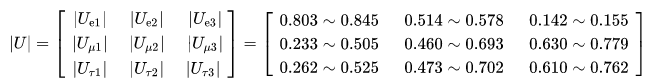
\includegraphics[width = \linewidth]{umn/pmns2022.png}
        \footnote{3$\sigma$ ranges of November 2022, From Wikipedia}
        \label{fig:enter-label}
    \end{figure}
\end{frame}

\begin{frame}{Sterile Neutrinos}
\begin{figure}
    \centering
    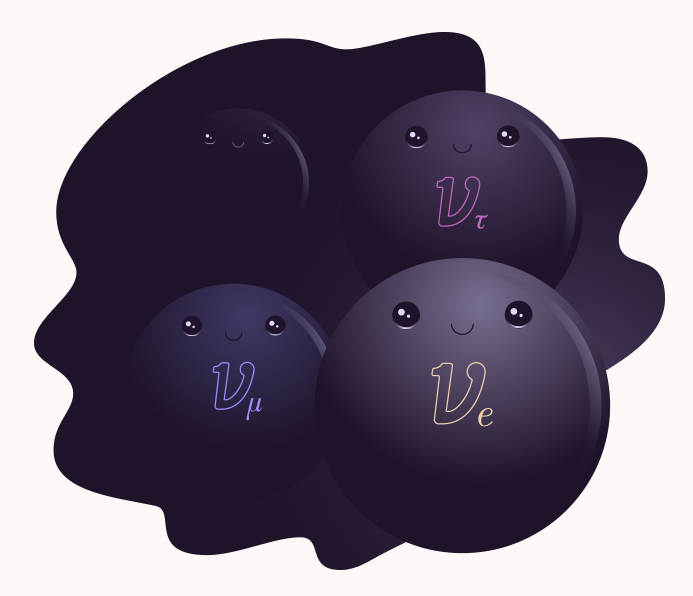
\includegraphics[width = 0.4\linewidth]{umn/sterile-neutrinos.jpg}
    \label{fig:sterile-neutrinos}
\end{figure} \pause

\begin{center}
    How can sterile neutrinos actually be observed?
\end{center}
\end{frame}

\begin{frame}{Detecting Sterile Neutrinos}
    \begin{itemize}
        \item LSND and MiniBooNE data seems to show anomalies (3-4 $\sigma$) \footnotesize[\cite{SBN-Paper}]\normalsize
        \vspace{0.5cm}
        \item Anomalies could be explained by a fourth, heavy $\nu$
        \vspace{0.5 cm}
        \item Null results from other experiments complicate things
    \end{itemize}
\end{frame}

\begin{frame}{Other Goals of SBN}
    \begin{itemize}
        \item Better understanding of neutrino-nucleus interactions \footnotesize[\cite{SBN-Paper}]\normalsize
        \vspace{0.5cm}
        \item Serve as precursor to DUNE
        \vspace{0.5cm}
        \item Milli-charged particles?
        \vspace{0.5cm}
        \item Dark matter candidates?
        \vspace{0.5cm}
        \item Other beyond-the-Standard-Model physics?
    \end{itemize} 
\end{frame}

\section{Experimental Setup}
\begin{frame}{Making a $\nu_{\mu}$ beam}
    \begin{figure}
        \centering
        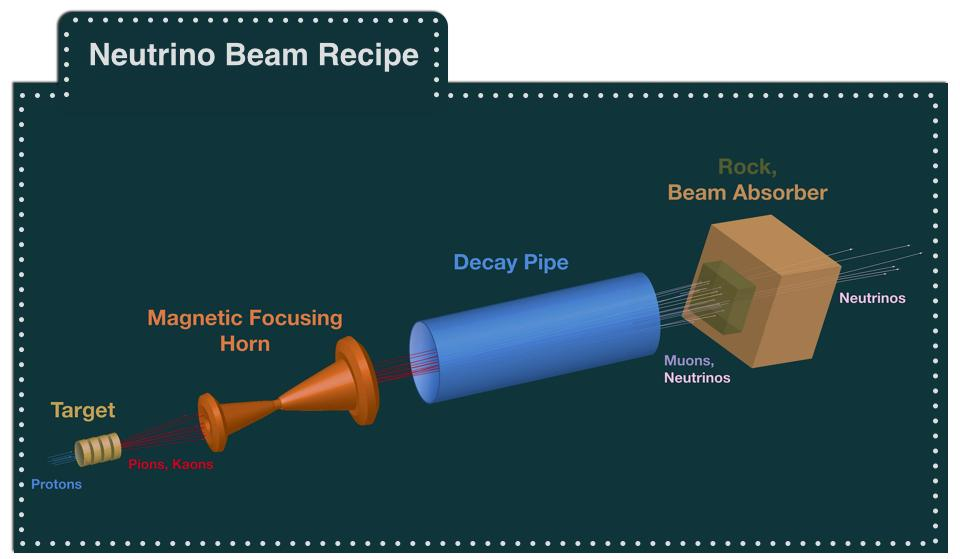
\includegraphics[width = \linewidth]{umn/fermilab-neutrino-beam.jpg}
        \label{fig:neutrino-beam}
    \end{figure}
    \vspace{-1 cm}
    \centering
    \footnotesize
    \cite{neutrino-beam}
    \normalsize
\end{frame}

\begin{frame}{Liquid Argon Time Projection Chambers (LArTPCs)}
    \onslide<1>\begin{itemize}
        \item A bubble chamber filled with liquid argon \footnotesize[\cite{ichep2018}]\normalsize
        \vspace{0.5 cm}
        \item Charged particles ionize argon, neutral particles don't (but can decay / interact)
        \vspace{0.5 cm}
        \item Electrode planes and photosensors allow 3-D reconstruction 
    \end{itemize}
    
    \onslide<2>
    \vspace{-3cm}
    \begin{figure}
        \centering
        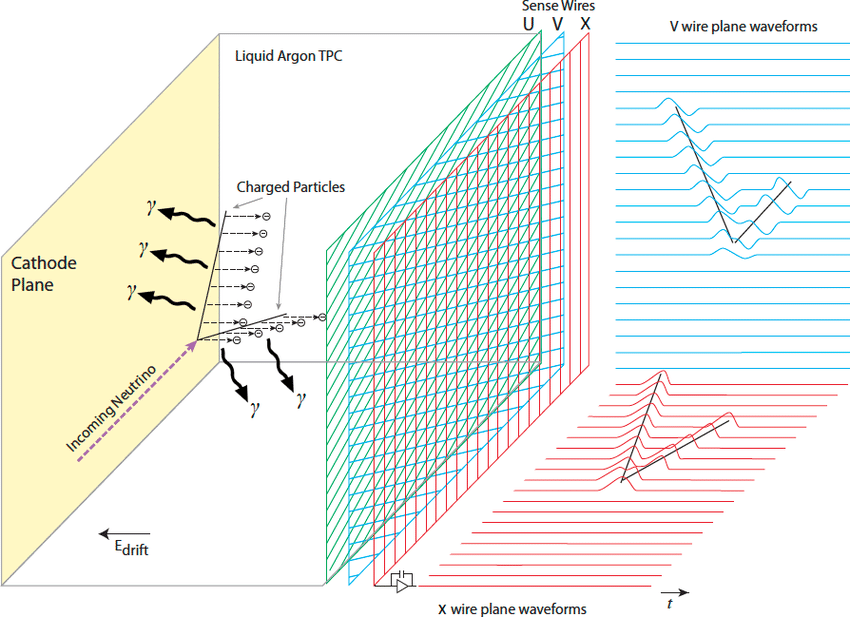
\includegraphics[width = 0.8\linewidth]{umn/lartpc.png}
        \label{fig:lartpc}
    \end{figure}
    \centering
    \tiny
    \cite{LArTPC}
\end{frame}

\begin{frame}{The SBN Detectors}
    \begin{figure}
        \centering
        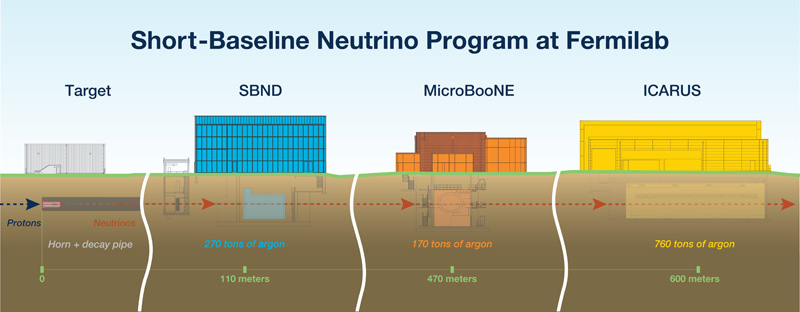
\includegraphics[width = \linewidth]{umn/sbn-detectors.png}
        \label{fig:sbn-detectors}
    \end{figure}
    \vspace{-1 cm}
    \centering
    \tiny
    \cite{sbn-diagram}
    \normalsize
\end{frame}

\section{Event Analysis}
\begin{frame}{Example of an Event}
    \begin{figure}
        \centering
        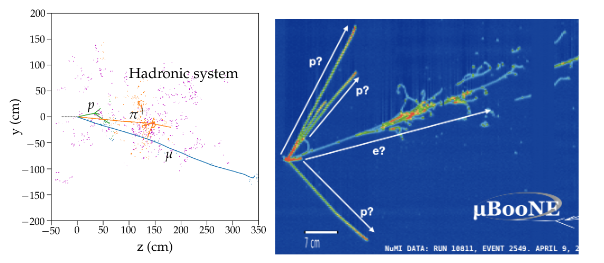
\includegraphics[width = \linewidth]{umn/microboone-tracks.png}
        \footnotesize
        \caption{LEFT: A 4 GeV $\nu_\mu$ simulated event in liquid argon.
        \vspace{0.25cm}
        
        RIGHT: Example of a candidate neutrino interaction in the MicroBooNE detector, displaying electromagnetic activity. \footnotesize[\cite{neutrino-snowmass}]\normalsize}
        \label{fig:microboone-tracks}
    \end{figure} 
\end{frame}

\begin{frame}{Some Analysis Notes}
    \begin{itemize}
         \item Analysis involves measurement of neutrino flavor rates at each SBN detector
        \vspace{0.5cm}
        \item Powerful algorithms reconstruct particle flavor \footnotesize[\cite{neutrino-snowmass}\normalsize]
        \vspace{0.5cm}
        \item LArTPC technology allows improvement over previous experiments \footnotesize[\cite{SBN-Paper}]\normalsize
        \vspace{0.5cm}
        \item Background includes cosmic rays, solar neutrinos
        \vspace{0.5cm}
        \item Having three (almost identical) detectors reduces systematic uncertainties
    \end{itemize}   
\end{frame}

\section{Summary and Conclusion}
\begin{frame}{In Summary}
    \begin{itemize}
        \item Neutrinos are a promising sector for new physics
        \vspace{0.5cm}
        \item Both a discovery and a precision machine
        \vspace{0.5 cm}
        \item Why I like SBN
        \vspace{0.5 cm}
        \item What I found challenging about SBN
    \end{itemize}
    
\end{frame}

\begin{frame}[t, allowframebreaks]
\frametitle{References}
    \printbibliography
\end{frame}

\end{document}